\section{Data generation}~\label{sec:htedata}
In ~\Cref{sec:pipeline}, a data-analysis pipeline is described to be applied on a relatively large sets of phase diagrams data described in~\Cref{sec:htedata}.
To derive the design rules we first perform dimensionality reduction followed by clustering. A overview of the dimensionality reduction and clustering methods can be found in~\ref{appendixB}.

The design space of variables are interaction parameter \(\chi\) values in~\Cref{eq:FH}.
The test case involves uniformly sampling the \(\chi\) values to be used in~\Cref{eq:FH} for a three component system. 
A uniform three-dimensional design space is defined via \(\chi_{12}\in[1.3,1.335,1.37,1.405,1.44]\) and 
\(\chi_{13}, \chi_{23}\in[0.3,0.6,1,1.5,2,2.5,3]\) a total of 245 phase diagrams are generated using the CEM method described in~\Cref{algo:cem}. 
The degree of polymerization for three materials are kept constant: $M_1=10$ for polymer, $M_2=10$ for small molecule, $M_3=1$ for solvent.
The goal using the model data set is to study the following question: \textit{given a densely sampled design space of phase diagram, can we automatically group various types of phase diagrams in the data set using clustering?}

\section{Data analysis pipeline}\label{sec:pipeline}
The data analysis pipeline as depicted in~\Cref{fig:mlpipeline} is as follows:~a) Generate a set of phase diagrams using the CEM in a high-throughput manner;~b) Compute pairwise similarities are and store in a matrix \(M\);~c) Apply clustering and dimensionality reduction to \(M\).
Spectral clustering method is used to obtain subgroups that are highly correlated within but not across using a Gaussian similarity of \(M\)~\cite{SpectralClustering}. 
A multi-dimensional scaling~(MDS)~\cite{ESL} of \(M\) is used to obtain a lower-dimensional representation using eigenvalues of \(M\) where each phase diagram can be represented using a point in a Cartesian coordinate system.
MDS and spectral clustering are performed using the \textit{scikit-learn}~\cite{sklearn} and other dependent python packages: scipy~\cite{scipy}, matplotlib~\cite{matplotlib} and mpltern~\cite{mpltern}.
Analyzing the lower dimensional representations and clustered subgroups together, allows users to decipher potential design rules that connect any two subgroups of phase diagrams. In \Cref{appendixB}, a detailed description of dimensionality reduction and clustering is provided with emphasis on geometrical interpretation of the methods used in this thesis.

The key element of the pipeline is the choice of the distance or similarity measure. The most commonly used distance is Euclidean norm, but other distances have been used~\cite{FiftySix}. 
In this work, we chose a \textit{Hamming} distance~(\Cref{eq:hamming}) between two grid-indexed representation of phase diagrams.

The point indexed phase diagram vectors are visualized by color-coding each point (instead of each simplex as before) in red (1-phase), green (2-phase) and blue (3-phase) as shown in (a) of~\Cref{fig:mlpipeline}.
The distance is then computed between a pair of phase label sets \(u,v\) indexed by composition using~\Cref{eq:hamming}.
\begin{equation}\label{eq:hamming}
    d(u,v) = \frac{1}{\ell}\sum_{i}\delta_{u[i],v[i]}
\end{equation}
where \(\delta_{ij}\) is the Kronecker-delta function and \(\ell\) is the cardinality of sets \(u,v\).
The Hamming distance is agnostic to the dimensionality of the grid \(G\), easy to compute thus making it a good choice for phase diagrams.  

\begin{figure}[h]
    \centering
    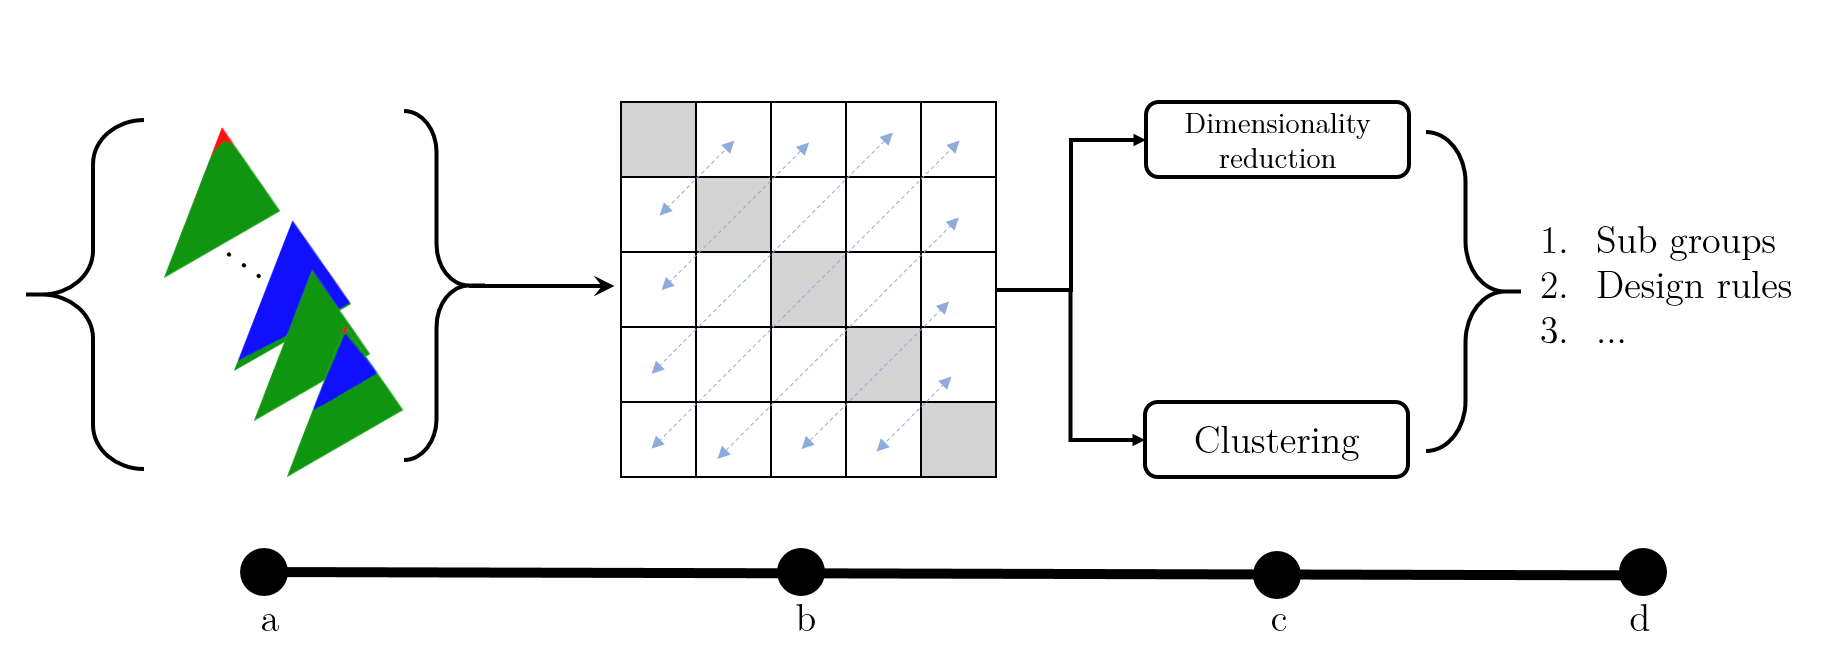
\includegraphics[width=\textwidth]{Chapter-4/figures/analysis_pipepline.png}
    \caption{Data analysis pipeline}
    \label{fig:mlpipeline}
\end{figure}

